\chapter{Neural-BO: A Black-box Optimization Algorithm using Deep Neural Networks} % Main chapter title
\label{chap:neural-bo}
\acfp{gp} are a popular probabilistic model for \ac{bo}. However, they are not well-suited for optimizing functions in complex, structured, high-dimensional spaces, such as those encountered in the optimization of images and text documents. This limitation arises because \acp{gp} rely on kernels to model functions, and widely used kernels, such as the Square Exponential and Mat\'ern kernels, struggle to accurately capture similarities within complex structured data. Consequently, \ac{bo} using \acp{gp} is limited in its applicability to fields like computer vision and natural language processing. Moreover, \acp{gp} face significant scalability challenges due to the cubic computational complexity of kernel inversion.

\acfp{dnn}, by contrast, have demonstrated exceptional scalability and generalization capabilities, particularly for high-dimensional and structured data. These qualities make them a potential alternative to \acp{gp} for optimization tasks. Recent efforts to leverage \acp{dnn} in black-box function optimization and contextual bandits have shown promise. However, many existing approaches depend on computationally expensive \acfp{bnn}, which require sampling-based methods to model predictive uncertainty, or they lack theoretical guarantees for convergence and sample efficiency.

To address these challenges, this chapter introduces Neural-BO, a novel framework for black-box optimization. In Neural-BO, the unknown function is modeled using an over-parameterized \ac{dnn}, eliminating the need for a \emph{\acf{bnn}} and making the algorithm computationally tractable. The framework leverages recent advances in neural network theory, particularly \acf{ntk}, to estimate confidence intervals around the neural network model. These confidence intervals are used within Thompson Sampling to draw random samples of the function, which are then maximized to determine the next evaluation point. We analyze the theoretical properties of Neural-BO, providing a regret bound that establishes its convergence and improved sample efficiency compared to existing methods. We summarize \textbf{the contributions of this chapter} as follows:

\begin{itemize}
    \item A deep neural network based black-box optimization algorithm (Neural-BO) that can perform efficient optimization by accurately modeling the complex structured data (e.g. image, text) and also being computationally favorable, i.e. scaling linearly with the number of data points.
    \item A theoretical analysis of our proposed Neural-BO algorithm showing that our algorithm is convergent with a sublinear regret bound. 
    \item Experiments with both synthetic benchmark optimization functions and real-world optimization tasks showing that our algorithm outperforms current state-of-the-art black-box optimization methods.
\end{itemize} 

This chapter begins with an outline of the problem setting and assumptions, followed by a detailed description of the Neural-BO framework and its theoretical analysis. 


\section{Problem Setting}
\label{section:neural-bo_problem_setting}
We consider a global optimization problem to maximize $f(\mathbf{x})$ subject to $\mathbf{x} \in \mathcal D \subset \mathbb{R}^d$, where $\mathbf{x}$ is the input with $d$ dimensions. The function $f$ is a noisy black-box function that can only be evaluated via noisy evaluations of $f$ in the form  $y= f(x) + \epsilon$, where $\epsilon$ is a sub-Gaussian noise which we will discuss more clearly in Assumption 2 in our regret analysis section. In our work, we consider input space $\mathcal D$ of the form: $a \leq \norm{\mathbf{x}}_2 \leq  b$,  where $a, b$ are absolute constants and $a \le b$. We note that this assumption is mild compared to current works in neural contextual bandits \citep{zhou2020neural,zhang2021neural,xu2020neural,kassraie2022neural} that required $\norm{\mathbf{x}}_2 = 1$.  


\section{Proposed Neural-BO Method}
\label{section:neural-bo_proposed_method}
In this section, we present our proposed \ac{dnn}-based black-box algorithm, Neural-BO. Following the principle of \ac{bo}, our algorithm consists of two main steps: (1) build a model of the black-box objective function, and (2) use the black-box model to choose the next function evaluation point at each iteration. For the first step, unlike traditional BO algorithms which use \ac{gp} to model the objective function, our idea is to use a fully connected neural network $h(\mathbf{x}; \boldsymbol{\theta})$ to learn the function $f$ as follows:
$$ h(\mathbf{x};\boldsymbol{\theta}) = \sqrt{m} \mathbf{W}_L \phi(\mathbf{W}_{L-1}\phi(\cdots\phi(\mathbf{W}_1 \mathbf{x})), $$
where $\phi(x) = \max(x,0)$ is the \ac{relu} activation function, $\mathbf{W}_1 \in \mathbb{R}^{m \times d}, \mathbf{W}_i \in \mathbb{R}^{m \times m}, 2\leq i \leq L-1, \mathbf{W}_L \in \mathbb{R}^{1 \times m}$, and $\boldsymbol{\theta} = (vec(\mathbf{W}_1),\cdots, vec(\mathbf{W}_L)) \in \mathbb{R}^p$ is the collection of parameters of the neural network, $p=md+m^2(L-2)+m$. To make the analysis tractable, we assume that the width $m$ is the same for all hidden layers. We also denote the gradient of the neural network by $\mathbf{g}(\mathbf{x}; \boldsymbol{\theta}) = \nabla_{\boldsymbol{\theta}}h(\mathbf{x}; \boldsymbol{\theta}) \in \mathbb{R}^p$.

For the second step, we choose the next sample point $\mathbf{x}_t$ by using a Thompson Sampling strategy. In particular, given each $\mathbf{x}$, our algorithm maintains a Gaussian distribution for $f(\mathbf{x})$. To choose the next point, it samples a random function $\widetilde{f}_t$ from the posterior distribution $\mathcal{N}(h(\mathbf{x}, \boldsymbol{\theta}_{t-1}), \nu_t^2 \sigma^2_t (\mathbf{x}))$, where 
\begin{align*}
\sigma^2_t (\mathbf{x}) &= \lambda \mathbf{g}(\mathbf{x};\boldsymbol{\theta}_0)\mathbf{U}_{t-1}^{-1}\mathbf{g}(\mathbf{x};\boldsymbol{\theta}_0)
\\
\mathbf{U}_{t-1} &= \sum_{i=0}^{t-1} \mathbf{g}(\mathbf{x}_i;\boldsymbol{\theta}_0)\mathbf{g}(\mathbf{x}_i; \boldsymbol{\theta}_0)^\top/m,
\end{align*}
and $\nu_t = \sqrt{2}B +\frac{R}{\sqrt{\lambda}} \sqrt{2 \log(1/ \delta)}$. From here, $\sigma_t(\mathbf{x})$ and $\nu_t$ construct a confidence interval, where for all $\mathbf{x} \in \mathcal{D}$, we have $\lvert  f(\mathbf{x}) - f(\mathbf{x}, \boldsymbol{\theta}) \rvert \leq \nu_t\sigma_t(\mathbf{x})$ that holds with probability $1-\delta$. We also note the difference from \citet{zhang2021neural} that uses $\mathbf{g}(\mathbf{x};\boldsymbol{\theta}_t)/\sqrt{m}$ as dynamic feature map, we here use a fixed feature map $\mathbf{g}(\mathbf{x};\boldsymbol{\theta}_0)/\sqrt{m}$ which can be viewed as a finite approximation of the feature map $\phi(\mathbf{x})$ of $k_\textup{NTK}$. This allows us to eliminate $\sqrt{m}$ away the regret bound of our algorithm. Then, the next evaluation is selected as $\mathbf{x}_t = \argmax_{\mathbf{x} \in \mathcal{D}} \widetilde{f_t}(\mathbf{x})$. 

% where $D_t$ is the  decision set which is chosen as a suitable discretization of the search space $\mathcal D$ at each iteration $t$. For technical reasons which can be seen in the proof of Lemma \ref{lemma:sampling_bound}, we specify $D_t$ at the beginning of Section \ref{sec:regret_analysis}. 

Besides, to initialize the network $h(\mathbf{x}; \boldsymbol{\theta}_0)$, we randomly generate each element of $\boldsymbol{\theta}_0$ from an appropriate Gaussian distribution: for each $1 \leq l \leq L-1$, each entry of $\mathbf{W}$ is generated from $\mathcal N(0, 2/m)$ independently; while each entry of the last layer $\mathbf{W}_L$ is set to zero to make $h(\mathbf{x}, \boldsymbol{\theta}_0) = 0$. Here we inherit so-called \emph{He initialization} \citep{he2015delving}, which ensures the stability of the expected length of the output vector at each hidden layer. 

The proposed Neural-BO is summarized using Algorithm \ref{alg:Neural-BO} and Algorithm \ref{alg:train_NN}. In section \ref{section:neural-bo_regret_analysis}, we will demonstrate that our algorithm can achieve a sublinear regret bound, and works well in practice (See our section \ref{section:neural-bo_experiments}).
\paragraph{Discussion}
A simple way to have a \ac{dnn}-based black-box algorithm is to extend the existing works of \citet{zhou2020neural,zhang2021neural} or \citet{kassraie2022neural} to our setting where the search space is continuous. However, this is difficult because these algorithms are designed for a finite set of actions. A simple adaptation can yield non-vanishing bounds on cumulative regret. For example, the regret bound in \citet{kassraie2022neural} depends on the size of finite action spaces $\lvert \mathcal A \rvert$. If $\lvert \mathcal A \rvert \rightarrow \infty$ then the regret bound goes to infinity. In \citet{zhou2020neural,zhang2021neural}, the regret bounds are built on gram matrix $\mathbf{H}$ which is defined through the set of actions. However, such a matrix cannot even be defined in our setting where the search space (action space) is infinite. We solve this challenge by using a discretization of the search space at each iteration as mentioned in Section \ref{section:neural-bo_regret_analysis}. In addition, for our confidence bound calculation, using $\mathbf{g}(\mathbf{x};\boldsymbol{\theta}_0)/\sqrt{m}$ instead of $\mathbf{g}(\mathbf{x};\boldsymbol{\theta}_t)/\sqrt{m}$ as in \citet{zhou2020neural,zhang2021neural} allows us to reduce a factor $\sqrt{m}$ from our regret bound.    

Our algorithm is also different from \citet{chowdhury2017kernelized} in traditional Bayesian optimization which uses a Gaussian process to model the function with posterior computed in closed form. In contrast, our algorithm computes posterior by gradient descent. 

\begin{algorithm}[]
\caption{Neural Black-box Optimization (Neural-BO)}
\label{alg:Neural-BO}
\textbf{Input}: The input space $\mathcal D$, the number of rounds $T$, exploration parameter $\nu_t$, network width $m$, RKHS norm bound $B$, regularization parameter $\lambda$, $\delta \in (0,1)$.
\begin{algorithmic}[1]
\State Set $\mathbf{U}_0 = \lambda \mathbf{I}$ 

\For{$t = 1$ to $T$}
    % \State Set $\nu_t = B + R\sqrt{ \log(1+\lambda^{-1}(t-1))\widetilde{d}_{t-1}  + 2 + 2 \log(1/ \delta)}$
\State $\sigma^2_t (\mathbf{x}) = \lambda \mathbf{g}(\mathbf{x};\boldsymbol{\theta}_0)^\top\mathbf{U}_{t-1}^{-1}\mathbf{g}(\mathbf{x};\boldsymbol{\theta}_0)/m$ \label{line:calculate_var}

\State $\widetilde{f_t}(\mathbf{x}) \sim \mathcal{N}(h(\mathbf{x}; \boldsymbol{\theta}_{t-1}), \nu_t^2 \sigma^2_t(\mathbf{x}))$ 
\State Choose $\mathbf{x}_t = \argmax_{\mathbf{x} \in \mathcal{D}} \widetilde{f_t}(\mathbf{x}) $ and receive observation $y_t = f(\mathbf{x}_t) + \epsilon_t$ 
   
\State Update $\boldsymbol{\theta}_t \leftarrow \text{TrainNN}(\{\mathbf{x}_i\}^t_{i=1} \{y_i\}^t_{i=1}, \boldsymbol{\theta}_0)$ \label{line:train_NN}
\State $\mathbf{U}_t \leftarrow \mathbf{U}_{t-1} +  \frac{\mathbf{g}(\mathbf{x}_t;\boldsymbol{\theta}_0)\mathbf{g}(\mathbf{x}_t; \boldsymbol{\theta}_0)^\top}{m} $ \label{line:update_Ut}
\EndFor
\end{algorithmic}
\end{algorithm}

\begin{algorithm}[H]
\caption{TrainNN}
\label{alg:train_NN}
\textbf{Input}: Chosen points $\{\mathbf{x}_i\}^t_{i=1}$, noisy observations $\{y_i\}^t_{i=1}$, initial parameter $\boldsymbol{\theta}_0$, number of gradient descent steps $J$, regularization parameter $\lambda$, network width $m$, learning rate $\eta$.
\begin{algorithmic}[1]
\State Define objective function $\mathcal{L}(\boldsymbol{\theta})  = \frac{1}{2}\sum^T_{i=1} (f(\mathbf{x}_i; \boldsymbol{\theta}) - y_i)^2 + \frac{1}{2}m\lambda\norm{\boldsymbol{\theta} - \boldsymbol{\theta}^{(0)}}^2_2$
\For{$k=0,\cdots ,J-1$}

$\boldsymbol{\theta}^{(k+1)} = \boldsymbol{\theta}^{(k)} - \eta \nabla \mathcal{L}(\boldsymbol{\theta}^{(k)})$
\EndFor

\State Return $\boldsymbol{\theta}^{(J)}$.
\end{algorithmic}
\end{algorithm}


\section{Theoretical Analysis}
\label{section:neural-bo_regret_analysis}

In this section, we provide a regret bound for the proposed Neural-BO algorithm. Our regret analysis is built upon the recent advances in \ac{ntk} theory \citep{allen2019convergence, cao2019generalization} and proof techniques of \ac{gp}-\ac{ts} \citep{chowdhury2017kernelized}. 
Unlike most previous neural-based contextual bandits works \citep{zhang2021neural, zhou2020neural} that restrict necessarily the search space to a set $\mathbb{S}^{d-1} = \{ \mathbf{x} \in \mathbb {R}^d \colon \norm{\mathbf{x}}_2 = 1 \}$, we here derive our results for a flexible condition, where the norms of inputs are bounded: $a \leq \norm{\mathbf{x}}_2 \leq b, \text{where } 0 < a \le b$. 

For theoretical guarantees, we need to use the following definition and assumptions on the observations $\mathcal{D}_t = \{\mathbf{x}_i, y_i\}^T_{i=1}$.


\begin{definition} [\cite{jacot2018neural}]
\label{def:NTK_matrix}
Consider the same set $\mathcal{D}_t$ as above and define

\[ \widetilde{\mathbf{H}}_{i,j}^{(1)} = \mathbf{\Sigma}_{i,j}^{(1)} = \langle  \mathbf{x}_i, \mathbf{x}_j \rangle\ , \mathbf{A}_{i,j}^{(l)} = 
\begin{pmatrix}
\mathbf{\Sigma}_{i,i}^{(l)} & \mathbf{\Sigma}_{i,j}^{(l)} 
\\
\mathbf{\Sigma}_{i,j}^{(l)} & \mathbf{\Sigma}_{j,j}^{(l)}
\end{pmatrix}\] 

\[\mathbf{\Sigma}_{i,j}^{(l+1)} = 2 \mathbb{E}_{(u,v) \sim \mathbf{N}(\mathbf{0}, \mathbf{A}_{i,j}^{(l)})} [\phi(u) \phi(v)] \]

\[ \widetilde{\mathbf{H}}_{i,j}^{(l+1)} = 2\widetilde{\mathbf{H}}_{i,j}^{(l)}\mathbb{E}_{(u,v) \sim \mathbf{N}(\mathbf{0}, \mathbf{A}_{i,j}^{(l)}} [\phi^\prime(u) \phi^\prime(v)] + \mathbf{\Sigma}_{i,j}^{(l+1)}, \]
where $\phi(\cdot)$ is the activation function of the neural network $h(\mathbf{x}; \boldsymbol{\theta})$.
Then $\mathbf{H}_t = \frac{\mathbf{\widetilde{H}}^{(L)}+ \mathbf{\Sigma} ^ {(L)}}{2}$ is called the NTK matrix on the set $\mathcal{D}_t$. 
\end{definition}


\begin{assumption} \label{assumption:sufficient_exploration} There exists $\lambda_0 > 0$, 
$\mathbf{H}_T \ge \lambda_0 \mathbf{I}_T$.
\end{assumption}
This is a common assumption in the literature \citep{zhou2020neural,xu2020neural,zhang2021neural}, and is satisfied as long as we sufficiently explore the input space such that no two inputs $\mathbf{x}$ and $\mathbf{x}^\prime$ are identical.  

\begin{assumption}
    We assume the objective function $f$ is from a \ac{rkhs} (See Section \ref{background:rkhs}) corresponding to a positive definite \ac{ntk}  $k_\text{NTK}$. In particular, $\norm{f}_{\mathcal{H}_{k_\text{NTK}}} \leq B$, for a finite $B > 0$. These assumptions indicate the smoothness of function $f$ and are regular as they have been typically used in many previous works \citep{chowdhury2017kernelized, srinivas2009gaussian,vakili2021information}.
\end{assumption}
\begin{assumption}
\label{assumption:iid_noise}
We assume the noises $\{\epsilon_i\}_{i=1}^T$ where $\epsilon_i = y_i - f(\mathbf{x}_i)$, are i.i.d and sub-Gaussian with parameter $R > 0$ and are independent with $\{\mathbf{x}_i\}_{i=1}^T$. 
%We also assume that the noise sequence $\{\epsilon_i\}_{i=1}^T$  are independent of $\{\mathbf{x}_i\}_{i=1}^T$. 
\end{assumption} 
This assumption is mild and similar to the work of \citet{vakili2021optimal} where the assumption is used to prove an optimal order of the regret bound for Gaussian process bandits. We use it here to provide a regret bound with the sublinear order for our proposed algorithm.    

Now we are ready to bound the regret of our proposed Neural-BO algorithm. To measure the regret of the algorithm, we use the cumulative regret which is defined as follows: $R_T = \sum_{t=1}^T r_t $ after $T$ iterations, where $\mathbf{x}^* = \argmax_{\mathbf{x} \in \mathcal{D}} f(\mathbf{x}) $ is the maximum point of the unknown function $f$ and $r_t = f(\mathbf{x^*}) - f(\mathbf{x}_t)$ is instantaneous regret incurred at time $t$. For further details on cumulative regret and its role as a performance metric, refer to Section \ref{background:performance_metrics}. We present our main theoretical result.
\begin{theorem}
\label{theorem:neural-bo_main} Let $\delta \in (0,1)$. Assume that the true underlying $f$ lies in the RKHS $\mathcal{H}_{k_\textup{NTK}}(\mathcal D)$ corresponding
to the NTK kernel $k_{\textup{NTK}}(\mathbf{x}, \mathbf{x'})$ with RKHS norm bounded by $B$.
Set the parameters in Algorithm \ref{alg:Neural-BO}
as $\lambda = 1 + \frac{1}{T}$, $\nu_t = \sqrt{2}B +\frac{R}{\sqrt{\lambda}}( \sqrt{2 \log(1/ \delta)}$, where $R$ is the noise sub-Gaussianity parameter.  
Set $\eta = (m\lambda + mLT)^{-1}$ and $J = (1+ LT /\lambda) \left(1+ \log(T^3L\lambda^{-1}\log \left(1/ \delta \right))\right)$. If the network width m satisfies:
\[ m \geq \textup{poly}\left(\lambda, T, \log(1/\delta), \lambda_0^{-1}\right),\]
then with probability at least $1-\delta$, the regret of Algorithm \ref{alg:Neural-BO} is bounded as

\begin{flalign*}
R_T & \leq C_1(1+c_T)\nu_T \sqrt{L} \sqrt{\frac{\lambda BT}{\log(B+1)} (2\gamma_T+1)}  \\
     & +  (4+  C_2(1+c_T)\nu_T L)\sqrt{2 \log(1/\delta)T} + \frac{(2B+1)\pi^2}{6} + \frac{b(a^2+b^2)}{a^3}
\end{flalign*} 
where $C_1, C_2$ are absolute constants, $a$ and $b$ are lower and upper norm bounds of $\mathbf{x} \in \mathcal{D}$  and $c_T=\sqrt{4\log T + 2 \log \ \lvert \mathcal D_t \rvert}$.
\end{theorem}
\remark{There exists a component $\frac{b(a^2 + b^2)}{a^3}$ in the regret bound $R_T$. This component comes from the condition of the search space. If we remove the influence
of constants $a,b, B$ and $R$, Theorem \ref{theorem:neural-bo_main} implies that our regret bound follows an order $\widetilde{O}( \sqrt{T\gamma_T})$. This regret bound has the same order as the one of the Maximum Variance Reduction algorithm in \citet{vakili2021optimal}, but is significantly better than traditional BO algorithms (e.g., \citep{srinivas2009gaussian, chowdhury2017kernelized}) 
 and existing neural contextual bandits (e.g., \citep{zhou2020neural,zhang2021neural}) that have the order $\widetilde{O}(\gamma_T\sqrt{T})$.  We note that the regret bounds in \citet{zhou2020neural,zhang2021neural} are expressed through the effective dimension $\widetilde{d} = \frac{ \log \det (\mathbf{I} + \mathbf{H}/\lambda)}{\log(1 + TK/\lambda)}$, where $K$ is the number of arm in contextual bandits setting. However, $\gamma_T$ and the effective dimension are of the same order up to a ratio of $1/(2 \text{log} (1 + TK/\lambda))$. The improvement of factor $\sqrt{\gamma_T}$ is significant because for \ac{ntk} kernel as shown by \citet{kassraie2022neural}, $\gamma_T$ follows order $\mathcal{O}(T^{1-1/d})$, where $d$ is the input dimension. For $d \ge 2$, existing bounds become vacuous and are no longer sublinear. In contrast, our regret bound remains sublinear for any $d>0$.} 


 \section{Proof of the Main Theorem}
To perform analysis for continuous actions as in our setting, we use a discretization technique. At each time $t$, we use a discretization $\mathcal{D}_t \subset \mathcal{D}$ with the property that $\lvert f(\mathbf{x}) - f([\mathbf{x}]_t) \rvert \leq \frac{1}{t^2}$ where $[\mathbf{x}]_t \in \mathcal{D}_t$ is the closest point to $\mathbf{x} \in \mathcal{D}$. Then we choose $\mathcal{D}_t $ 
with size $\lvert \mathcal{D}_t \rvert = \left( (b-a)BC_{\text{lip}}t^2 \right)^d$ that satisfies $\norm{\mathbf{x} - [\mathbf{x}]_t}_1 \leq \frac{b-a}{(b-a)BC_{\text{lip}}t^2} = \frac{1}{BC_{\text{lip}}t^2}$ for all $\mathbf{x} \in \mathcal{D}$,
where $C_{\text{lip}}= \underset{\mathbf{x} \in \mathcal{D}} {\supremum} \underset{j \in [d]} {\supremum} \left( \frac{\partial^2 k_\text{NTK}(\mathbf{p},\mathbf{q})}{\partial \mathbf{p}_j \mathbf{q}_j} \lvert \mathbf{p}=\mathbf{q}=\mathbf{x} \right)$. This implies, for all $\mathbf{x} \in \mathcal{D}$:
\begin{equation}
\label{eqn:rkhs_lipschitz}
    \lvert f(\mathbf{x}) - f([\mathbf{x}]_t) \rvert \leq \norm{f}_{\mathcal{H}_{k_\textup{NTK}}} C_{\text{lip}} \norm{\mathbf{x} - [\mathbf{x}]_t}_1 \leq BC_{\text{lip}} \frac{1}{BC_{\text{lip}}t^2} =  1/t^2, 
\end{equation}
is Lipschitz continuous of any $f \in \mathcal{H}_{k_\textup{NTK}}(\mathcal{D})$ with Lipschitz constant $B C_{\text{lip}}$, where we have used our assumption $\norm{f}_{\mathcal{H}_{k_\textup{NTK}}} \leq B$. We bound the regret of the proposed algorithm by starting from the instantaneous regret $r_t = f(\mathbf{x}^*) - f(\mathbf{x}_t)$ can be decomposed to $r_t = [f(\mathbf{x}^*) - f([\mathbf{x}^*]_t)] + [f([\mathbf{x}^*]_t - f(\mathbf{x}_t)]$. While the first term is bounded by Eqn. (\ref{eqn:rkhs_lipschitz}),  we bound the second term in Lemma \ref{lemma:neural-bo_regret_bound} provided in our Appendix. The proof of Lemma \ref{lemma:neural-bo_regret_bound} requires a few steps, namely (a) introduce a saturated set $\mathcal S_t$ (see Definition \ref{def:saturated_set}), then combine it with the results of Lemma \ref{lemma:sampling_bound} (deriving a bound on $\lvert \widetilde{f}_t(\mathbf{x}) - h(\mathbf{x}; \boldsymbol{\theta}_{t-1}) \rvert$) necessitated due to the Thompson sampling and Lemma \ref{lemma:predictive_bound} (deriving a bound on $\lvert f(\mathbf{x}) - h(\mathbf{x}; \boldsymbol{\theta}_{t-1}) \rvert$) utilizing the generalization result of the over-parameterized neural networks. Note that, in our proof, we consider the effect of our general search space setting (where input $\mathbf{x} \in \mathcal{D}$ is norm-bounded, i.e.,  $0 < a \le \norm{\mathbf{x}}_2 \le b$) on the output of the over-parameterized deep neural network at each layer in Lemma \ref{lemma:bound_hil} and on the gradient of this network utilized in Lemma \ref{lemma:NN_vs_linear}. These results contribute to the appearance of the lower and the upper norm bounds $a$ and $b$, the first in the generalization property of over-parameterized neural networks in Lemma \ref{lemma:predictive_bound} and the latter affect the cumulative regret bound in Theorem \ref{theorem:neural-bo_main}. Our proof follows the proof style of Lemma 4.1 of \citet{cao2019generalization}, Lemma B.3 of \citet{cao2019generalization} and Theorem 5 
of \citet{allen2019convergence}. 

On the other hand, Lemma \ref{lemma:noise_affeted_bound}, based on Assumption \ref{assumption:iid_noise}, provides a tighter bound on the confidence interval that eliminated the factor $\sqrt{\gamma_T}$, in comparison with previous relevant works \citet{chowdhury2017kernelized, zhou2020neural}, leading to the sublinear regret bound in Theorem \ref{theorem:neural-bo_main}.   
By these arguments, we achieve a cumulative regret bound for our proposed algorithm in terms of the maximum information gain $\gamma_T$ (Lemma \ref{lemma:neural-bo_regret_expectation}, \ref{lemma:neural-bo_regret_bound}, \ref{lemma:min_sigma}). \textbf{Our detailed proof is provided in Appendix \ref{section:neural-bo_appendix}}.

% after introducing saturated set $\mathcal{S}_t$ in Definition \ref{def:saturated_set} and achieving the bound for $\lvert f(\mathbf{x}) - h(\mathbf{x}; \boldsymbol{\theta}_{t-1}) \rvert$ using Gaussian concentration in Lemma \ref{lemma:sampling_bound} due to the sampling process in  Algorithm \ref{alg:Neural-BO} and $\lvert \widetilde{f}_t(\mathbf{x}) - h(\mathbf{x}; \boldsymbol{\theta}_{t-1}) \rvert$ in Lemma \ref{lemma:predictive_bound}, utilizing the generalization result of the trained over-parameterized neural network after $T$ rounds. 



\begin{proof} [Proof Sketch for Theorem \ref{theorem:neural-bo_main}]
\label{proof:theorem_main}
% Because Lemma \ref{lemma:predictive_bound} holds with probability at least $1-\delta$. Then, w
With probability at least $1-\delta$, we have
% \begin{equation*}
% \begin{split}
\begin{align*}
 R_T &  = \sum^T_{t=1} f(\mathbf{x^*}) - f(\mathbf{x}_t) \\ 
     % & = \sum^T_{t=1} (f(\mathbf{x^*}) - f(\mathbf{x}_t)
     % \\ 
     & = \sum^T_{t=1} \left[f(\mathbf{x}^*) - f([\mathbf{x}^*]_t)\right] + \left[f([\mathbf{x}^*]_t) - f(\mathbf{x}_t) \right] \\ 
     &\leq 4T \epsilon(m) + \frac{(2B+1)\pi^2}{6} + \Bar{C}_1(1+c_T)\nu_T \sqrt{L} \sum^T_{i=1} \min(\sigma_t(\mathbf{x}_t), B) \\
     & \quad +(4+\Bar{C}_2(1+c_T)\nu_T L + 4\epsilon(m))\sqrt{2 \log(1/\delta)T} \\
     & \leq \Bar{C}_1 (1+c_T)\nu_T \sqrt{L} \sqrt{\frac{\lambda BT}{\log(B+1)} (2\gamma_T+1)} 
     + \frac{(2B+1)\pi^2}{6} + 4T \epsilon(m) \\
     & \quad + 4\epsilon(m)\sqrt{2 \log(1/\delta)T}  +  \left(4+\Bar{C}_2(1+c_T)\nu_T L\right)\sqrt{2 \log(1/\delta)T}  \\
     &  = \Bar{C}_1(1+c_T)\nu_t \sqrt{L} \sqrt{\frac{\lambda BT}{\log(B+1)} (2\gamma_T+1)} + \frac{(2B+1)\pi^2}{6} \\
     & \quad +  \epsilon(m)(4T+ \sqrt{2 \log(1/\delta)T}) + (4+\Bar{C}_2(1+c_T)\nu_t L)\sqrt{2 \log(1/\delta)T} \\
     \end{align*} 
The first inequality is due to Lemma \ref{lemma:neural-bo_regret_bound}, which provides the bound for cumulative regret $R_T$ in terms of $\sum^T_{t=1} \min(\sigma_t(\mathbf{x}_t),B)$.  The second inequality further provides the bound of term $\sum^T_{t=1} \min(\sigma_t(\mathbf{x}_t),B)$ due to Lemma \ref{lemma:min_sigma}, while the last equality rearranges addition.  Picking
\begin{align*}
    \eta &= (m\lambda + mLT)^{-1} \text{ and}
    \\
    J & = \left(1+LT/\lambda \right) \left(\log (C_{\epsilon,2} ) + \log(T^3L\lambda^{-1}\log(1/\delta)) \right),
\end{align*}
we have 
\begin{equation*}
\begin{split}
      &\frac{b}{a} C_{\epsilon,2}(1 - \eta m \lambda)^J \sqrt{TL/\lambda} \left(4T+\sqrt{2 \log(1/\delta)T}\right)\\
    = & \frac{b}{a} C_{\epsilon,2} \left(1-\frac{1}{1+LT/\lambda}\right)^{J} \left(4T+\sqrt{2 \log(1/\delta)T}\right) \\
    = & \frac{b}{a} C_{\epsilon,2} e^{-\left(\log \left(C_{\epsilon,2}\right) + \log(T^3L\lambda^{-1}\log(1/\delta)) \right)} \left(4T+\sqrt{2 \log(1/\delta)T}\right)\\
    = & \frac{b}{a}  \frac{1}{C_{\epsilon,2}}.T^{-3}L^{-1}\lambda \log^{-1}(1/\delta) \left(4T+\sqrt{2 \log(1/\delta)T}\right)  \le   \frac{b}{a}\\
\end{split}
\end{equation*}
Then choosing $m$ that satisfies:
\begin{equation*}
    \begin{split}
        \left(\frac{b}{a} C_{\epsilon,1} m^{-1/6}\lambda^{-2/3}L^3 \sqrt{\log m} + \left(\frac{b}{a}\right)^3 C_{\epsilon,3} m^{-1/6} \sqrt{\log m} L^4 T^{5/3} \lambda^{-5/3} (1+\sqrt{T/\lambda})\right) \\
        \left(4T+  \sqrt{2 \log(1/\delta)T}\right) \le \left(\frac{b}{a}\right)^3 
    \end{split}
\end{equation*}
We finally achieve the bound of $R_T$ as:
\begin{flalign*}
R_T & \leq \Bar C_1(1+c_T)\nu_T \sqrt{L} \sqrt{\frac{\lambda BT}{\log(B+1)} (2\gamma_T+1)}  \\
     & +  (4+ \bar C_2(1+c_T)\nu_T L)\sqrt{2 \log(1/\delta)T} + \frac{(2B+1)\pi^2}{6} + \frac{b(a^2+b^2)}{a^3}
\end{flalign*}
\end{proof}
\section{Experiments}
\label{section:neural-bo_experiments}

In this section, we demonstrate the effectiveness of our proposed Neural-BO algorithm compared to traditional BO algorithms and several other BO algorithms on various synthetic benchmark optimization functions and various real-world optimization problems that have complex and structured inputs. The real-world optimization problems consist of (1) generating sensitive samples to detect tampered model trained on MNIST \citep{lecun-mnisthandwrittendigit-2010} dataset; (2) optimizing control parameters for robot pushing considered in \citet{wang2017max}; and (3) optimizing the number of evaluations needed to find a document that resembles an intended (unknown) target document.
\subsection{Experimental Setup}
For all experiments, we compared our algorithm with common classes of surrogate models used in black-box optimization, including \acp{gp}, \acp{rf} and \acp{dnn}. For \acp{gp}, we have three baselines: GP-UCB \citep{srinivas2009gaussian}, GP-TS \citep{chowdhury2017kernelized} and GP-EI \citep{jones1998efficient} with the common Squared Exponential (SE) kernel. Our implementations for GP-based Bayesian Optimization baselines utilize public library GPyTorch\footnote{\url{https://gpytorch.ai/}} and BOTorch\footnote{\url{https://botorch.org/}}. Next, we consider SMAC \citep{hutter2011sequential} as a baseline using \ac{rf} as a surrogate model. Lastly, we also include two recent \acp{dnn}-based works for black-box optimization: DNGO \citep{snoek2015scalable} and Neural Greedy \citep{pariagreedy}. We further describe the implementations for \ac{rf} and \ac{dnn}-based baselines as follows: 
\begin{itemize}
    \item \ac{rf}-based surrogate model is implemented using public library GPyOpt\footnote{\url{https://github.com/SheffieldML/GPyOpt}} and optimization is performed with EI acquisition function.
    \item DNGO \citep{snoek2015scalable} models the black-box function by a Bayesian linear regressor, using low-dimensional features (extracted by DNN) as inputs. We run DNGO algorithm with the implementation of AutoML\footnote{\url{https://github.com/automl/pybnn}} with default settings. 
    \item NeuralGreedy \citep{pariagreedy} fits a neural network to the current set of observations, where the function values are randomly perturbed before learning the neural network. The learned neural network is then used as the acquisition function to determine the next query point. Our re-implementation of NeuralGreedy follows the setting described in Appendix F.2 \citep{pariagreedy}.  
\end{itemize}
 

%\subsubsection{Neural-BO implementation details}
For our proposed Neural-BO algorithm, we model the functions using two-layer neural networks $f(\mathbf{x}; \boldsymbol{\theta}) = \sqrt{m}\mathbf{W}_2\sigma(\mathbf{W}_1\mathbf{x})$ with network width $m=500$. 
The weights of the network are initialized with independent samples from a normal distribution $\mathcal{N} (0, 1/m)$. To train the surrogate neural network models, we use SGD optimizer with batch size 50, epochs 50, learning rate $\eta=0.001$ and regularizer $\lambda=0.01$. We set exploration parameter in Algorithm \ref{alg:Neural-BO}: $\nu_t = \nu$ and do a grid search over $\{0.1,1,10\}$. 

\subsection{Synthetic Benchmarks}
We optimized several commonly used synthetic benchmark functions: Ackley, Levy, and Michalewics. The exact expression of these functions can be found at: \url{http://www.sfu.ca/~ssurjano/optimization.html}. To emphasize the adaptation of our method to various dimensions, for each function, we performed optimization for four different dimensions, including 10, 20, 50, and 100. This is done to evaluate the methods across a range of dimensions. The function evaluation noise follows a normal distribution with zero mean and the variance is set to 1\% of the function range.
\begin{figure}[]
    \centering
    \begin{subfigure}[b]{\textwidth}
        \centering
        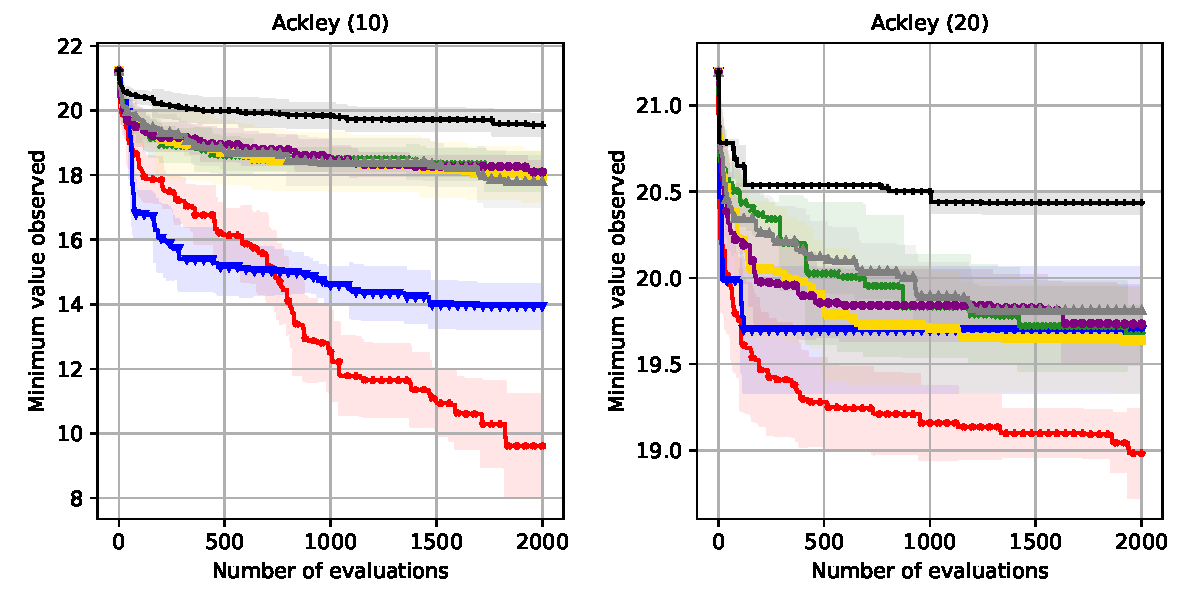
\includegraphics[width=\textwidth]{Figures/Neural-BO/A1.pdf}
    \end{subfigure}
    \begin{subfigure}[b]{\textwidth}
        \centering
        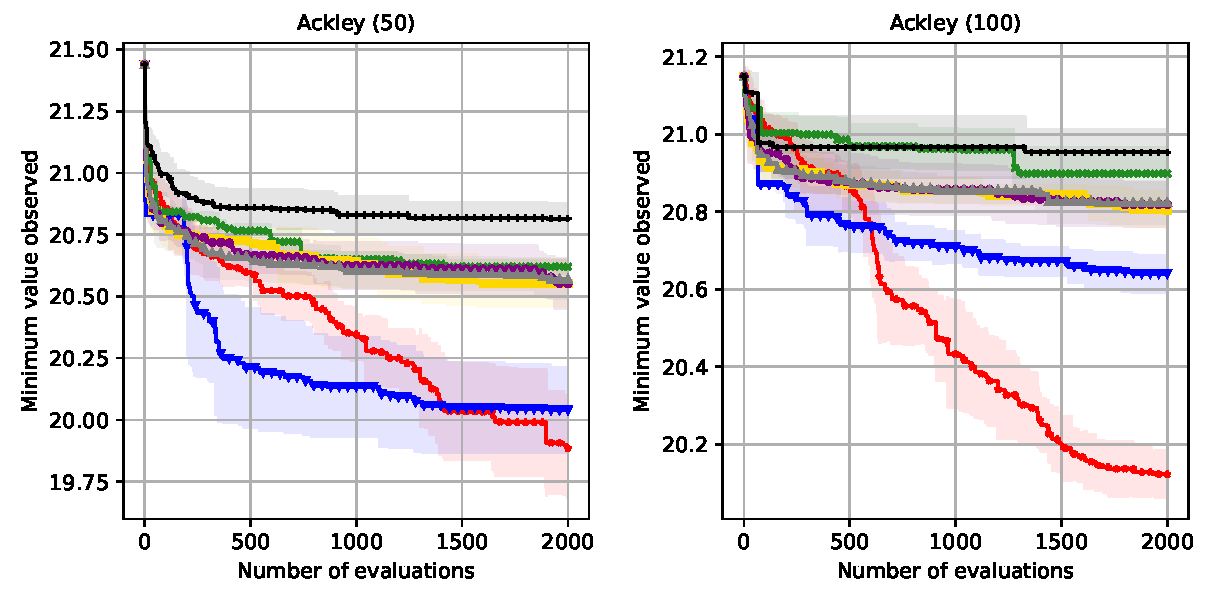
\includegraphics[width=\textwidth]{Figures/Neural-BO/A2.pdf}
    \end{subfigure}
    \begin{subfigure}[b]{\textwidth}
        \centering
        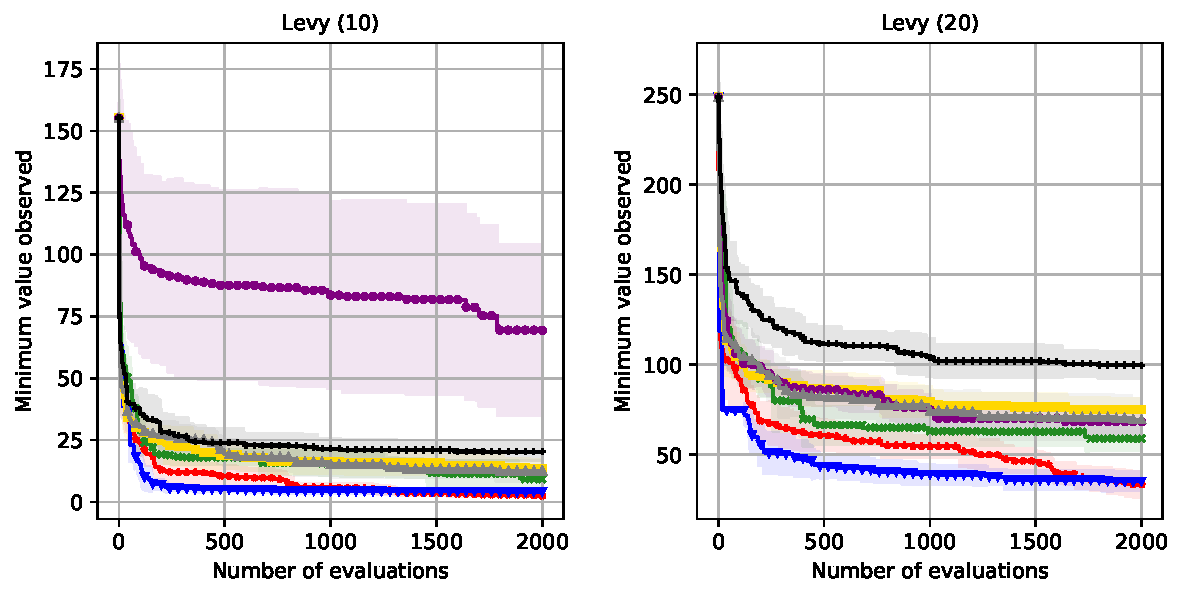
\includegraphics[width=\textwidth]{Figures/Neural-BO/L1.pdf}
    \end{subfigure}
    \label{fig:neural-bo_synthetic_1}
\end{figure}


\begin{figure}[]
    \centering
    \ContinuedFloat
    \begin{subfigure}[b]{\textwidth}
        \centering
        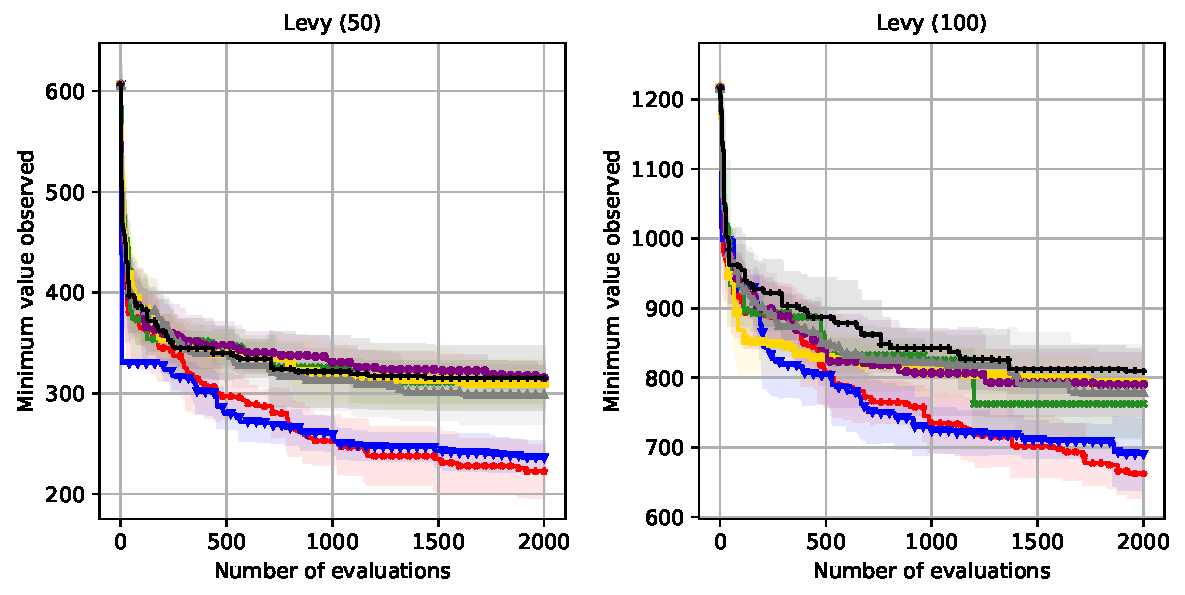
\includegraphics[width=\textwidth]{Figures/Neural-BO/L2.pdf}
    \end{subfigure}
    \begin{subfigure}[b]{\textwidth}
        \centering
        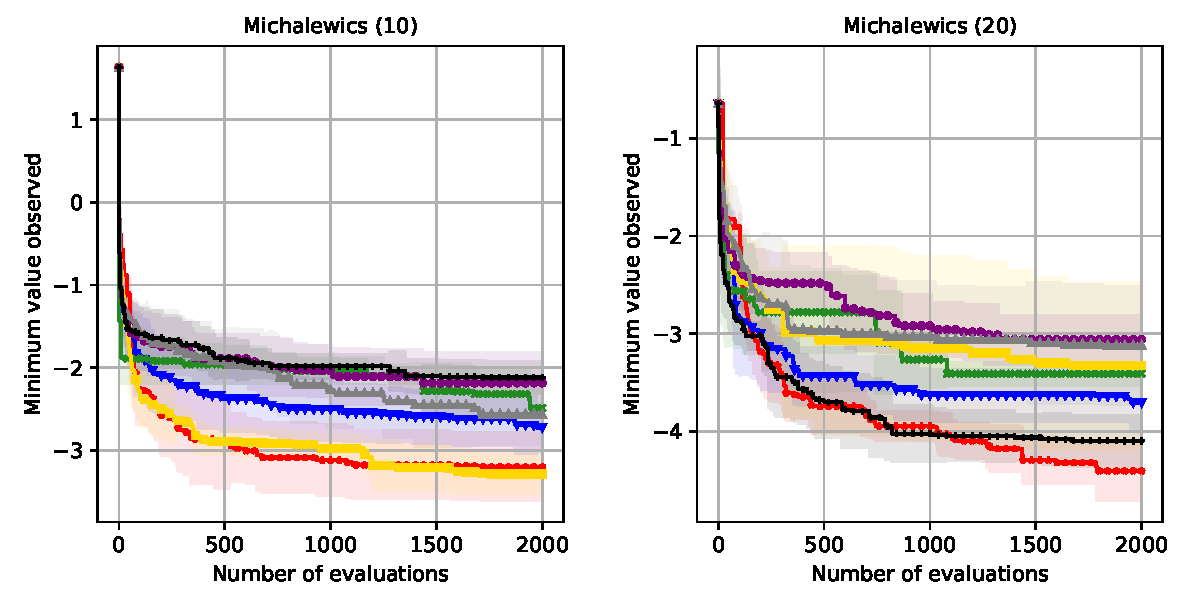
\includegraphics[width=\textwidth]{Figures/Neural-BO/M1.pdf}
    \end{subfigure}
    \begin{subfigure}[b]{\textwidth}
        \centering
        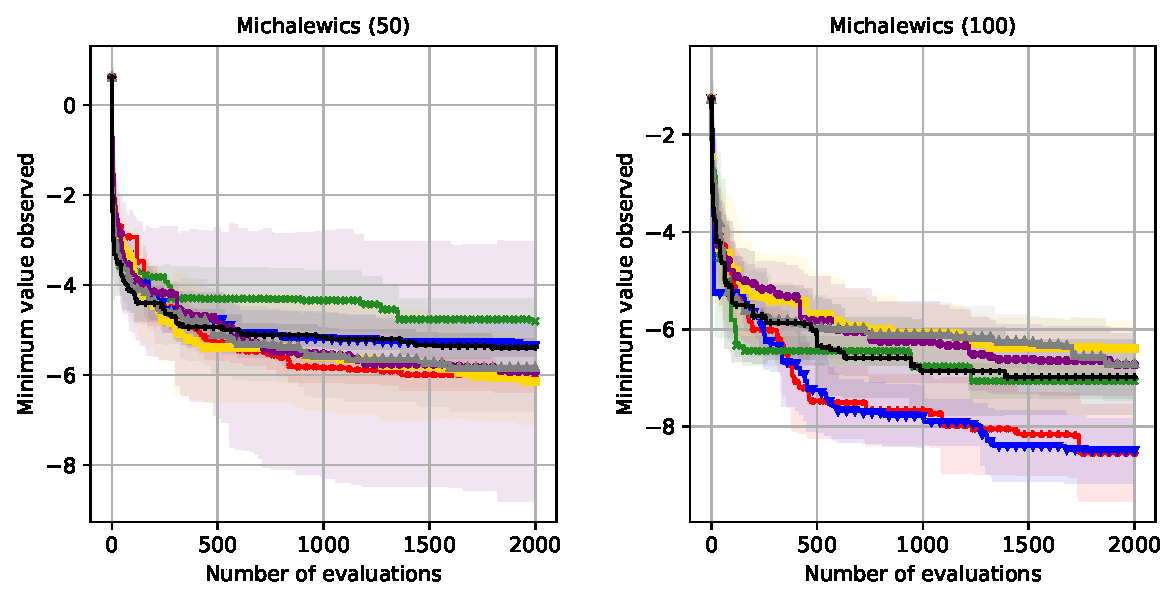
\includegraphics[width=\textwidth]{Figures/Neural-BO/M2.pdf}
    \end{subfigure}
    \begin{subfigure}[b]{0.8\textwidth}
        \centering
        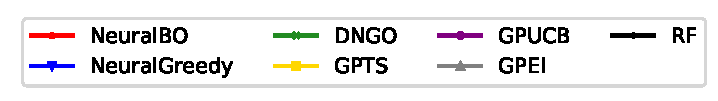
\includegraphics[width=\textwidth]{Figures/Neural-BO/baselines.pdf}
    \end{subfigure}
    \caption{The plots show the minimum true value observed after optimizing several synthetic functions over 2000 iterations of our proposed algorithm and 6 baselines. The dimension of each function is shown in the parenthesis.}
    \label{fig:neural-bo_synthetic}
\end{figure}




All reported experiments are averaged over 10 runs, each using a random initialization. All the methods start with the same set of initial points. As seen from Figure \ref{fig:neural-bo_synthetic}, Neural-BO is comparable to or better than all other baselines, including GP-based BO algorithms, both NN-based BO algorithms (DNGO and NeuralGreedy) and one algorithm using random forest. Moreover, our algorithm is also promising for high dimensions. 



In order to assess the statistical significance of whether our proposed method outperforms all baselines, we conducted a series of tests. First, a Kolmogorov-Smirnov (KS) test was performed to check if the sample sets for the hypothesis test follow a normal distribution. The null hypothesis assumes no difference between the observed and normal distribution. The p-values obtained from the KS test are presented in Table \ref{tab:ks_test}.  As all p-values exceeded 0.05, we failed to reject the null hypothesis, indicating that all data can be considered as normally distributed. Subsequently, one-sided t-tests were employed (as the variance is unknown), along with the Benjamini-Hochberg correction for multiple hypotheses testing, for each pair of (baseline, Neural-BO). These tests aimed to determine whether the baseline achieves a lower objective function value than our proposed method, Neural-BO. The alternative hypothesis $H_a: \mu_\text{baseline} > \mu_{\text{Neural-BO}}$ was tested against the null hypothesis $H_0: \mu_\text{baseline} \le \mu_{\text{Neural-BO}}$. Detailed test results are provided in Table \ref{tab:t-test}, where each cell contains two values: the first value represents the p-value obtained from the t-test, and the second value (T or F) indicates the outcome of the Benjamini-Hochberg correction where "T" indicates that the null hypothesis is rejected, whereas an "F" indicates that it is not rejected.







\begin{table}[]
\resizebox{\textwidth}{!}{
\begin{tabular}{|cc|c|c|c|c|c|c|c|}
\hline
\multicolumn{2}{|c|}{}                                                                                          & \textbf{\begin{tabular}[c]{@{}c@{}}Neural\\-BO\end{tabular}} & \textbf{\begin{tabular}[c]{@{}c@{}}Neural\\ Greedy\end{tabular}} & \textbf{\begin{tabular}[c]{@{}c@{}}GP\\-UCB\end{tabular}} & \textbf{\begin{tabular}[c]{@{}c@{}}GP\\-TS\end{tabular}} & \textbf{\begin{tabular}[c]{@{}c@{}}GP\\-EI\end{tabular}} & \textbf{DNGO} & \textbf{RF} \\ \hline
\multicolumn{1}{|c|}{\multirow{4}{*}{\textbf{Ackley}}}                                                  & D=10  & 0.85                                                         & 0.83                                                             & 0.95                                                      & 0.95                                                     & 0.45                                                     & 0.23          & 0.79        \\ \cline{2-9} 
\multicolumn{1}{|c|}{}                                                                                  & D=20  & 0.31                                                         & 0.46                                                             & 0.91                                                      & 0.90                                                     & 1.00                                                     & 1.00          & 0.93        \\ \cline{2-9} 
\multicolumn{1}{|c|}{}                                                                                  & D=50  & 0.95                                                         & 0.38                                                             & 0.81                                                      & 0.99                                                     & 0.52                                                     & 0.85          & 0.67        \\ \cline{2-9} 
\multicolumn{1}{|c|}{}                                                                                  & D=100 & 0.84                                                         & 0.77                                                             & 0.94                                                      & 0.82                                                     & 0.82                                                     & 0.38          & 0.97        \\ \hline
\multicolumn{1}{|c|}{\multirow{4}{*}{\textbf{Levy}}}                                                    & D=10  & 0.75                                                         & 0.45                                                             & 0.79                                                      & 0.72                                                     & 0.72                                                     & 0.58          & 0.63        \\ \cline{2-9} 
\multicolumn{1}{|c|}{}                                                                                  & D=20  & 0.84                                                         & 1.00                                                             & 1.00                                                      & 0.79                                                     & 0.79                                                     & 0.91          & 0.89        \\ \cline{2-9} 
\multicolumn{1}{|c|}{}                                                                                  & D=50  & 0.76                                                         & 0.34                                                             & 0.75                                                      & 0.75                                                     & 0.98                                                     & 0.77          & 0.37        \\ \cline{2-9} 
\multicolumn{1}{|c|}{}                                                                                  & D=100 & 0.76                                                         & 0.59                                                             & 0.87                                                      & 0.90                                                     & 0.99                                                     & 0.93          & 0.95        \\ \hline
\multicolumn{1}{|c|}{\multirow{4}{*}{\textbf{\begin{tabular}[c]{@{}c@{}}Micha-\\ lewics\end{tabular}}}} & D=10  & 0.54                                                         & 0.56                                                             & 0.95                                                      & 0.88                                                     & 0.83                                                     & 0.77          & 0.55        \\ \cline{2-9} 
\multicolumn{1}{|c|}{}                                                                                  & D=20  & 0.60                                                         & 0.99                                                             & 0.43                                                      & 0.33                                                     & 0.31                                                     & 0.56          & 0.85        \\ \cline{2-9} 
\multicolumn{1}{|c|}{}                                                                                  & D=50  & 0.90                                                         & 0.80                                                             & 0.64                                                      & 0.39                                                     & 0.68                                                     & 0.99          & 0.95        \\ \cline{2-9} 
\multicolumn{1}{|c|}{}                                                                                  & D=100 & 0.70                                                         & 0.58                                                             & 0.96                                                      & 0.57                                                     & 0.96                                                     & 0.93          & 0.52        \\ \hline
\end{tabular}
}
\caption{The p-values of KS-test "whether the data obtained from running our methods Neural-BO and all baselines are normally distributed".}
\label{tab:ks_test}
\end{table}



% \begin{table}[H]
% \begin{tabular}{|c||c|c|c|}\hline
% \backslashbox[0.\linewidth]{DIM}{Obj}
% &\makebox[0.22\linewidth]{Ackley}&\makebox[0.22\linewidth]{Levy}&\makebox[0.22\linewidth]{Michalewics}\\\hline
% 10&(-7.51, 5.95e-14)&(-4.4, 1.06e-05)&(0.574, 0.566)\\\hline
% 20&(-4.99, 5.95e-07)&(-0.6, 0.548)&(-2.32, 0.0203)\\\hline
% 50&(-1.77, 0.0465)&(-1.35, 0.177)&(0.216, 0.829)\\\hline
% 100&(-20.2, 4.35e-91)&(-1.36, 0.175)&(-0.126, 0.899)\\\hline
% \end{tabular}
% \caption{The z-scores and p-values of the z-test "whether our proposed Neural-BO achieves lower function value than that of the runner-up baseline" for the synthetic function optimizations in Figure \ref{fig:synthetic}.}
% \label{tab:pvalue}
% \end{table}
\begin{table}[]
\resizebox{\textwidth}{!}{
\begin{tabular}{|cc|l|l|l|l|l|l|}
\hline
\multicolumn{2}{|c|}{}                                                                                          & \multicolumn{1}{c|}{\textbf{\begin{tabular}[c]{@{}c@{}}Neural\\ Greedy\end{tabular}}} & \multicolumn{1}{c|}{\textbf{GPUCB}} & \multicolumn{1}{c|}{\textbf{GPTS}} & \multicolumn{1}{c|}{\textbf{GPEI}} & \multicolumn{1}{c|}{\textbf{DNGO}} & \multicolumn{1}{c|}{\textbf{RF}} \\ \hline
\multicolumn{1}{|c|}{\multirow{4}{*}{\textbf{Ackley}}}                                                  & D=10  & (2.98e-07,   T)                                                                       & (3.11e-12, T)                       & (1.64e-11, T)                      & (2.3e-11, T)                       & (6.15e-09, T)                      & (2.09e-13, T)                    \\ \cline{2-8} 
\multicolumn{1}{|c|}{}                                                                                  & D=20  & (6.39e-05, T)                                                                         & (1.61e-06, T)                       & (4.72e-05, T)                      & (4.19e-08, T)                      & (0.000111, T)                      & (1.29e-05, T)                    \\ \cline{2-8} 
\multicolumn{1}{|c|}{}                                                                                  & D=50  & (0.0467, T)                                                                           & (2.23e-08, T)                       & (1.89e-08, T)                      & (8.5e-09, T)                       & (1.86e-08, T)                      & (2.11e-10, T)                    \\ \cline{2-8} 
\multicolumn{1}{|c|}{}                                                                                  & D=100 & (3.92e-14, T)                                                                         & (7.98e-16, T)                       & (2.43e-16, T)                      & (4.7e-16, T)                       & (6.44e-16, T)                      & (5.78e-17, T)                    \\ \hline
\multicolumn{1}{|c|}{\multirow{4}{*}{\textbf{Levy}}}                                                    & D=10  & (0.000171, T)                                                                         & (7.98e-06, T)                        & (8.81e-09, T)                      & (6.6e-07, T)                       & (1.68e-05, T)                      & (1.62e-11, T)                    \\ \cline{2-8} 
\multicolumn{1}{|c|}{}                                                                                  & D=20  & (0.278, F)                                                                            & (3.28e-09, T)                       & (4.32e-11, T)                      & (1.8e-07, T)                       & (4.75e-05, T)                      & (8.01e-14, T)                    \\ \cline{2-8} 
\multicolumn{1}{|c|}{}                                                                                  & D=50  & (0.0971, F)                                                                           & (5.37e-09, T)                       & (2.72e-07, T)                      & (6.47e-06, T)                      & (0.000188, T)                      & (1.99e-06, T)                    \\ \cline{2-8} 
\multicolumn{1}{|c|}{}                                                                                  & D=100 & (0.096, F)                                                                            & (1.09e-06, T)                       & (4.85e-08, T)                      & (9.87e-05, T)                      & (0.00456, T)                       & (5.57e-07, T)                    \\ \hline
\multicolumn{1}{|c|}{\multirow{4}{*}{\textbf{\begin{tabular}[c]{@{}c@{}}Micha-\\ lewics\end{tabular}}}} & D=10  & (5.9e-06, T)                                                                          & (7.79e-08, T)                       & (0.472, F)                         & (1.68e-05, T)                      & (7.49e-06, T)                      & (1.87e-11, T)                    \\ \cline{2-8} 
\multicolumn{1}{|c|}{}                                                                                  & D=20  & (2.63e-05, T)                                                                         & (3e-09, T)                          & (0.00108, T)                       & (1.02e-05, T)                      & (0.000163, T)                      & (0.0161, T)                      \\ \cline{2-8} 
\multicolumn{1}{|c|}{}                                                                                  & D=50  & (0.000344, T)                                                                         & (3.47e-06, T)                       & (0.315, F)                         & (0.101, F)                         & (0.000871, T)                      & (0.000132, T)                    \\ \cline{2-8} 
\multicolumn{1}{|c|}{}                                                                                  & D=100 & (0.45, F)                                                                             & (8.2e-05, T)                        & (8.49e-06, T)                      & (0.000126, T)                      & (0.0404, T)                        & (0.00579, T)                     \\ \hline
\end{tabular}
}
\caption{One-sided t-tests were employed to assess whether the baseline achieves a lower function value compared to our proposed method, Neural-BO.  The null hypothesis $H_0: \mu_\text{baseline} \le \mu_{\text{Neural-BO}}$ and the alternative hypothesis:  $H_a: \mu_\text{baseline} > \mu_{\text{Neural-BO}}$. The p-value corresponding to each test is provided as the first value in each cell. Moreover, to account for multiple hypotheses testing, the Benjamini-Hochberg correction was applied and is reported as the second value in each cell. In the outcome, a "T" indicates that the null hypothesis is rejected, whereas an "F" signifies that it is not rejected.}
\label{tab:t-test}
\end{table}


Next, we used the COmparing Continuous Optimizers (COCO) framework\footnote{ \url{https://github.com/numbbo/coco}} to compare the performance of our method with baseline methods. COCO is a widely used benchmarking platform for continuous optimization algorithms, providing researchers with a standardized set of test functions to evaluate different optimization methods. The framework includes a collection of test functions that are designed to be challenging to optimize and exhibit various properties, such as multimodality, ill-conditioning, or weak global structure. To evaluate our algorithms, we used the BBOB test functions, which consist of 24 noiseless, single-objective, and scalable functions. The quality indicator needs to reach or exceed a predefined target value  $t$  for COCO to consider a single run over a problem successful. The performance of different optimizers is measured by the \textit{Fraction of function, target pairs}, which indicates the ratio of problems solved at optimization step $T$. For more details on how COCO measures the performance of different optimizers, please refer to \citet{hansen2021coco}. We set the number of evaluations for our optimizers to be 20 times the dimension of the problem. 

\begin{figure}[]
\begin{subfigure}{.5\textwidth}
  \centering
  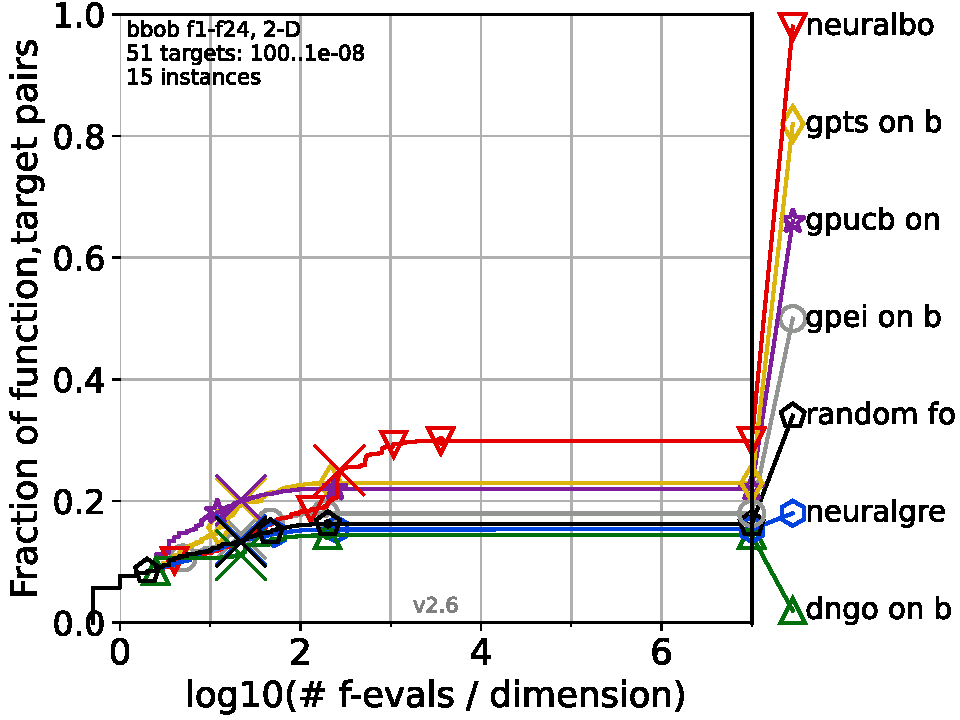
\includegraphics[width=\linewidth]{Figures/Neural-BO/Neural-BO_pprldmany_02D_noiselessall.pdf}
  \caption{2D}
  \label{fig:coco_2d}
\end{subfigure}%
\begin{subfigure}{.5\textwidth}
  \centering
  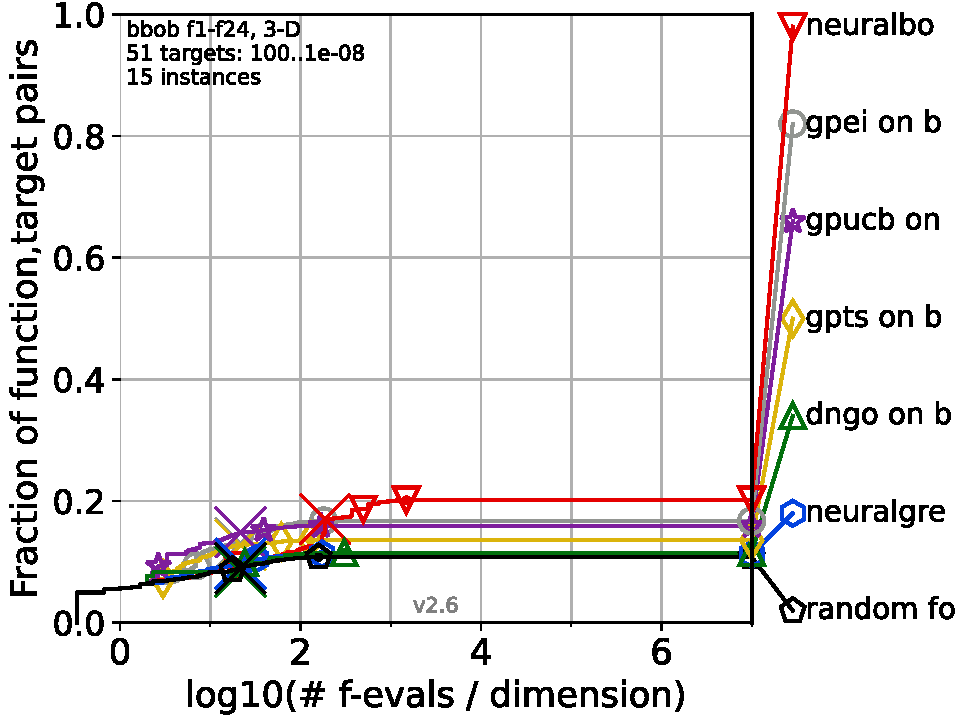
\includegraphics[width=\linewidth]{Figures/Neural-BO/Neural-BO_pprldmany_03D_noiselessall.pdf}
  \caption{3D}
  \label{fig:coco_3d}
\end{subfigure}
\begin{subfigure}{.5\textwidth}
  \centering
  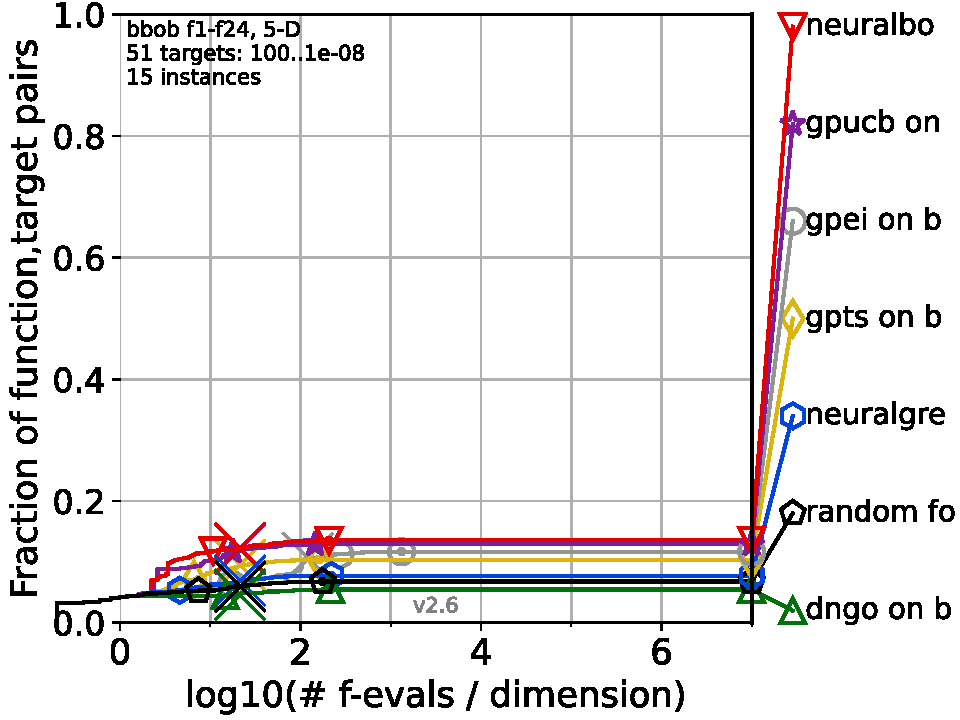
\includegraphics[width=\linewidth]{Figures/Neural-BO/Neural-BO_pprldmany_05D_noiselessall.pdf}
  \caption{5D}
  \label{fig:coco_5d}
\end{subfigure}%
\begin{subfigure}{.5\textwidth}
  \centering
  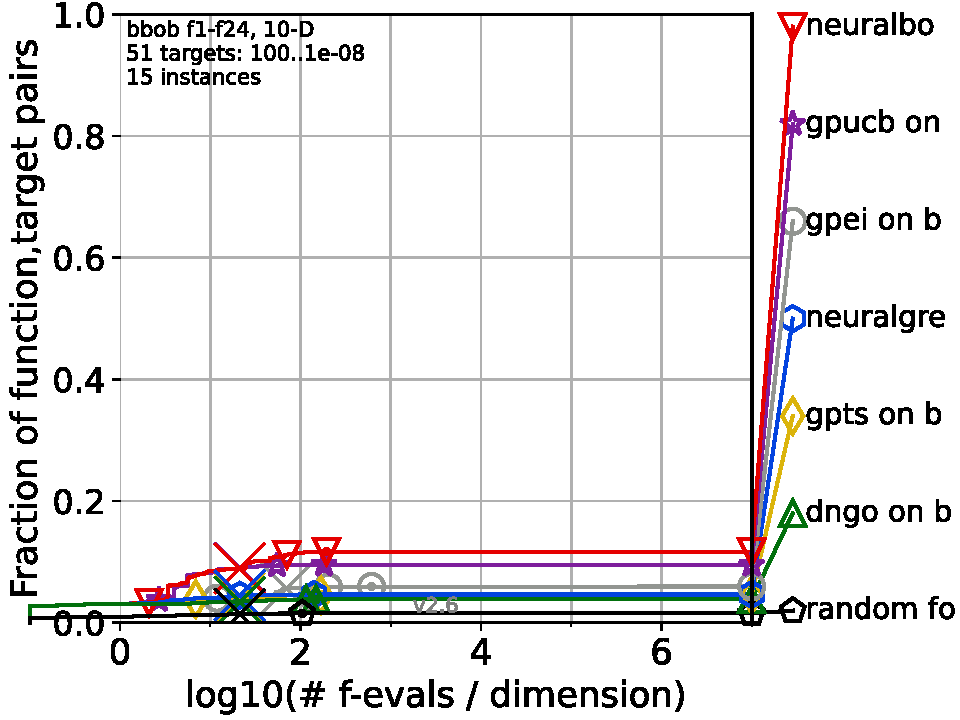
\includegraphics[width=\linewidth]{Figures/Neural-BO/Neural-BO_pprldmany_10D_noiselessall.pdf}
  \caption{10D}
  \label{fig:coco_10d}
\end{subfigure}
\caption{The results of benchmarking our Neural-BO and the baselines with COCO framework on 24 BBOB noiseless objective functions with four different dimensions \{2,3,5,10\}.}
\label{fig:coco}
\end{figure}

In Figure \ref{fig:coco}, we present the results of our experiment using the COCO benchmarking framework to evaluate all methods. The benchmarking comprised 24 noiseless functions with 15 instances, where each instance represented a unique condition of the function, such as the location of the optimum. Our method was found to outperform other baselines when assessed using the well-designed and publicly available COCO framework. 


\subsection{Real-world Applications}
\subsubsection{Designing Sensitive Samples for Detection of Model Tampering}
\label{section:neural-bo_sensitive_samples}
\begin{figure}[H]
    \centering
    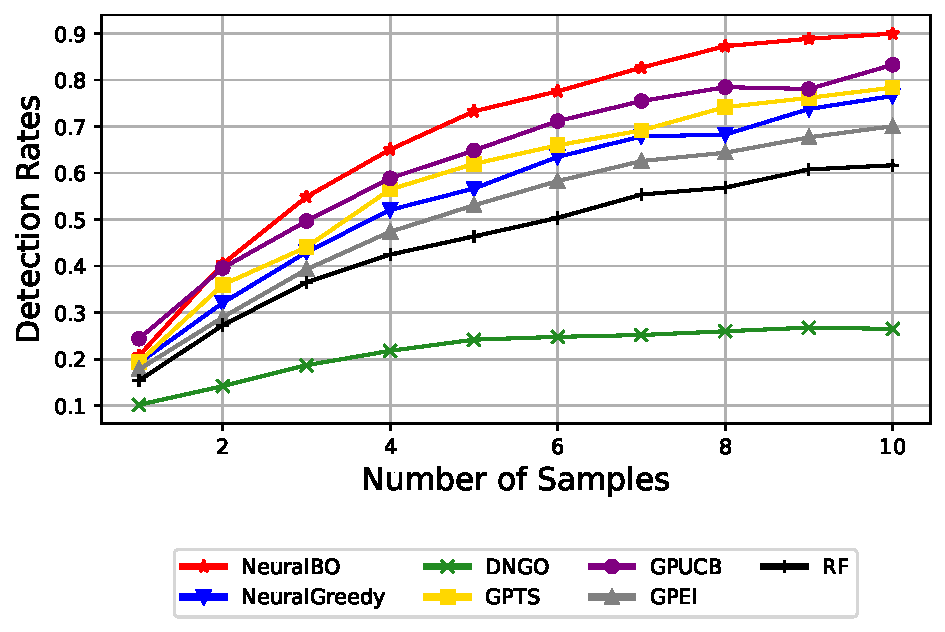
\includegraphics[width=\textwidth]{Figures/Neural-BO/Neural-BO_sensitive_sample_detection_rate.pdf}
    \caption{The plot shows the \textbf{detection rates} corresponding to the number of samples on the MNIST dataset. The larger the number of sensitive samples, the higher the detection rate. As shown in the figure, Neural-BO can generate sensitive samples that achieve nearly 90\% of the detection rate with at least 8 samples.}
    \label{fig:neural-bo_sensitive_sample}
\end{figure}

We consider an attack scenario where a company offering Machine Learning as a service (MLaaS) hosts its model on a cloud. However, an adversary with backdoor access may tamper with the model to change its weight. This requires the detection of model tampering. To deal with this problem, \citet{he2018verideep} suggests generating a set of test vectors named \emph{Sensitive-Samples} $\{v_i\}_{i=1}^n$, whose outputs predicted by the compromised model will be different from the outputs predicted by the original model. As formalized in \citet{he2018verideep}, suppose we suspect a pre-trained model $f_\theta(x)$ of having been modified by an attacker after it was sent to the cloud service provider. Finding sensitive samples for verifying the model's integrity is equivalent to optimizing task: $v = \argmax_x \norm{\frac{\partial f_\theta(x)}{\partial \theta}}_F$, where $\norm{\cdot}_F$ is the Frobenius norm of a matrix. A \emph{successful detection} is defined as ``given $N_S$ sensitive samples, there is at least one sample, whose top-1 label predicted by the compromised model is different from the top-1 label predicted by the correct model''. Clearly, optimizing this expensive function requires a BO algorithm to be able to work with high-dimensional structured images, unlike usual inputs that take values in hyper-rectangles.

We used a handwritten digit classification model (pre-trained on MNIST data) as the original model and tampered it by randomly adding noise to each weight of this model. We repeat this procedure 1000 times to generate 1000 different tampered models. The top-1 accuracy of the MNIST original model is $93\%$ and is reduced to $87.73\% \pm 0.08\%$ after modifications.   

To reduce the computations, we reduce the dimension of images from $28 \times 28$ to $7 \times 7$ and do the optimization process in 49-dimensional space. After finding the optimal points, we recover these points to the original dimension by applying an upscale operator to get sensitive samples. We compare our method with all other baselines by the average detection rate with respect to the number of sensitive samples. From Figure \ref{fig:sensitive_sample}, it can be seen that our method can generate  samples with better detection ability than other baselines. This demonstrates the ability of  our method to deal with complex structured data such as images. 

\subsubsection{Unknown target document retrieval}
\begin{figure}[H]
    \centering
    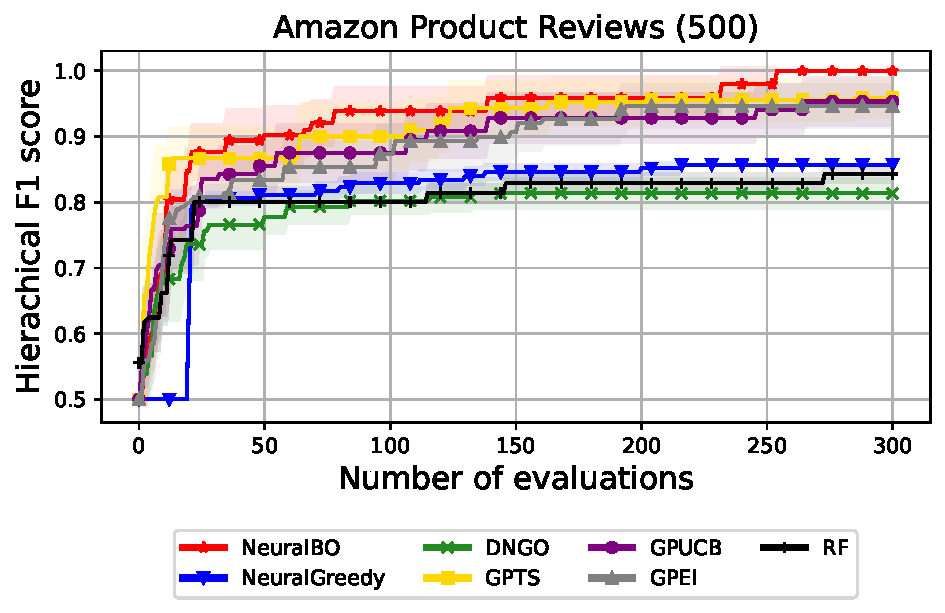
\includegraphics[width=\textwidth]{Figures/Neural-BO/Neural-BO_AmazonReview_dim_500_round_300.pdf}
    \caption{We search for the most related document for a specified target document in \textbf{Amazon product reviews} dataset and report the maximum \textbf{hierachical F1 score} found by all baselines. All methods show similar behaviour and Neural-BO performs comparably and much better than GP-based baselines.}
    \label{fig:text}
\end{figure}
Next, we evaluate our proposed method on a retrieval problem where our goal is to retrieve a document from a corpus that matches user's preference. The optimization algorithm works as follows: it retrieves a document, receives user's feedback score and then updates its belief and attempts again until it reaches a high score, or its budget is depleted. The objective target function is defined as the user’s evaluation of each document, which usually has a complex structure. It is clear that evaluations are expensive since the user must read each suggestion. Searching for the most relevant document is considered as finding document $d$ in the dataset $S_{text}$ that maximizes the match to the target document $d_t$: $d = \argmax_{d \in S_{text}} \textup{Match}(d, d_t)$, where $\textup{Match}(d, d_t)$ is a matching score between documents $d$ and $d_t$. We represent each document by a word frequency vector $x_{n} = (x_{n1}, \cdots, x_{nJ})$, where $x_{nj}$ is the number of occurrences of the $j$-th vocabulary term in the $n$-th document, and $J$ is the vocabulary size.  

Our experiment uses Amazon product reviews 
dataset\footnote{\url{https://www.kaggle.com/datasets/kashnitsky/hierarchical-text-classification}}, which are taken from users' product reviews from Amazon's online selling platform. This dataset has hierarchical categories, where the category classes are sorted from general to detail. The dataset is structured as: 6 classes in ``level 1'', 64 classes in ``level 2'' and 464 classes in ``level 3''. The number of users' reviews was originally 40K, which was reduced to 37738 after ignoring reviews with ``unknown'' category. We choose the size of vocabulary to be 500 and use the hierarchical F1-score introduced in  \citet{kiritchenko2005functional} as a scoring metric for the target and retrieved documents. We report the mean and standard deviation of hierarchical F1-score between target and retrieved documents over ten runs for all methods in Figure \ref{fig:text}. Figures \ref{fig:text} indicate that our method shows a better performance for the Amazon product review dataset in comparison with other approaches. 

\subsubsection{Optimizing control parameters for robot pushing} 
\begin{figure}[H]
    \centering
    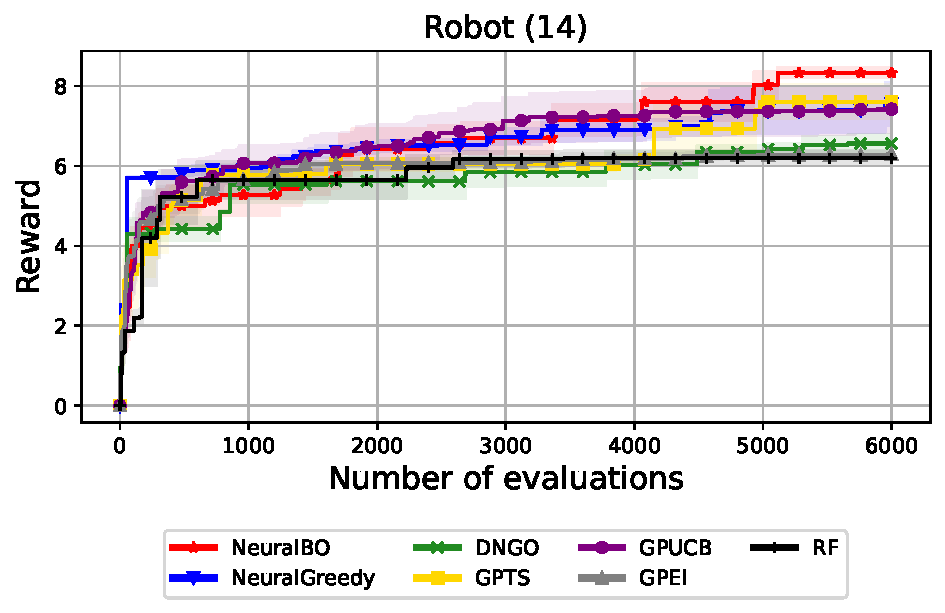
\includegraphics[width=\textwidth]{Figures/Neural-BO/Neural-BO_Robot_dim_14_round_6000.pdf}
    \vspace{-3mm}
    \caption{
    Optimization results for control parameters of 14D robot pushing problem. The X-axis shows iterations, and the y-axis shows the median of the best reward obtained.}
    \label{fig:robot_14D}
\end{figure}

Finally, we evaluate our method on tuning control parameters for the robot pushing problem considered in \citet{wang2017max}. We run each method for a total of 6000 evaluations and repeat ten times to take average optimization results. Neural-BO and all other methods are initialized with 15 points. Figure \ref{fig:robot_14D} summarizes the median of the best rewards achieved by all methods. It can be seen that Neural-BO achieves the highest reward after 5K optimization steps. 

\section{Conclusion}
We proposed a new algorithm for \acl{bo} using \aclp{dnn}. A key advantage of our algorithm is that it is computationally efficient and performs better than traditional \acl{gp} based methods, especially for complex structured design problems. We provided rigorous theoretical analysis for our proposed algorithm and showed that its cumulative regret converges with a sublinear regret bound. Using both synthetic benchmark optimization functions and a few real-world optimization tasks, we showed the effectiveness of our proposed algorithm. 